\chapter{Vorgehen}
\label{chap:vorgehen}

% Dieses Kapitel beschreibt das methodische Vorgehen, welches in der Arbeit angewendet wurde. Erwähnen Sie hier die verschiedenen Phasen der Arbeit und ihre Ergebnisse. Arbeiten mit hohem Softwareentwicklungs-Anteil lehnen sich am besten an eine etablierte Vorgehensweise an wie zum Beispiel Scrum, XP oder Agiler UP. Detailierte Projektpläne, Deliverables und anderes, falls vorhanden, gehören aber in den Anhang.
\section{Projektphasen}
\label{sec:projektphasen}

Um bei der Arbeit ein möglichst strukturiertes Vorgehen zu verfolgen, wurden folgende Projektphasen gewählt:
\begin{itemize}
\item Erarbeitung und Festhaltung der Anforderungen
\item Erarbeitung der formalen und technischen Grundlagen
\item Modellierung der Ontologie
\item Erstellung der Dokumentation zur Wissensmodellierung
\item Erarbeitung der praktischen Grundlagen
\item Erstellung der abschliessenden Dokumentation
\end{itemize}

Dabei ist zu sagen, dass die Phasen der Modellierung der Ontologie sowie der Erstellung der Dokumentation zur Wissensmodellierung grösstenteils parallel abliefen bzw. Hand in Hand übergingen. Die während der Modellierung erhaltenen Erkenntnisse konnten direkt in die Dokumentation übernommen werden. Die bei der Erarbeitung des Dokumentes erarbeiteten theoretischen Grundlagen konnten im Gegenzug direkt für die praktische Modellierung genutzt werden.

\subsection{Anforderungen}
\label{subsec:anforderungen}
In der Projektphase der Anforderungen wurden die Requirments an die Arbeit erarbeitet. Ergebnis dieser Phase ist ein Anforderungsdokument mit den wichtigsten Eckpunkten, siehe~\autoref{sec:anhang:anforderungen}. Es wurde ursprünglich festgehalten, dass der praktische Teil der Arbeit --- die Erarbeitung einer Ontologie anhand einer Wissensdomäne --- mittels eines konkreten Anwendungsproblems, der Erlernung der Programmiersprache Prolog, umgesetzt werden soll. 

Im Laufe der Arbeit hat sich jedoch gezeigt, dass semantische Netze bzw. Ontologien nicht ein geeignetes Mittel sind um Logiksprachen wie z.B. Prolog abzubilden. Dies wird Kapitel~\autoref{sub:modellierung_der_ontologie} genauer beschrieben.

\subsection{Formale und technische Grundlagen}
\label{sub:formale_und_technische_grundlagen}
Die formalen Grundlagen zur Modellierung der Ontologie sowie zur Erstellung der Dokumentation zur Wissensmodellierung waren teilweise bereits aufgrund des Vorprojektes --- BTI7302 -- Projekt 2, Details siehe~\autoref{sec:anhang:projekt2} --- vorhanden. Die restlichen formalen Grundlagen wurden anhand von~\cite{IspekOntoBedeutung},~\cite{ISpekOntoGeschichte},~\cite{w3sparql_querylang},~\cite{w3sparql_overview},~\cite{w3rdf_syntax},~\cite{w3rdf},~\cite{w3owl} und~\cite{swrl} erarbeitet.

Bedingt durch die oben erwähnte Vorarbeit, war das Konzept der technischen Umsetzung bereits gegeben. Es sollte aus zwei Komponenten, einem Backend --- in Form einer semantischen Datenbank, zur Verarbeitung von Anfragen an diese --- sowie einem Frontend --- zur einfachen Handhabung von Abfragen und der Ausgabe von Resultaten --- bestehen.

Wie schon in~\autoref{chap:Aufgabenstellung} erwähnt, fiel die ursprüngliche Wahl für das Backend auf Apache Stanbol~\url{http://stanbol.apache.org}, da dies alle Anforderungen zu erfüllen schien. Es stellte sich jedoch im Verlaufe der Arbeit heraus, dass dies nicht da geeignete Produkt für die geplante Umsetzung ist, Details siehe~\autoref{sec:komponenten}.

\subsection{Modellierung der Ontologie}
\label{sub:modellierung_der_ontologie}

\subsubsection{Vorarbeit fürs Modellierung der Ontologie}
\label{sub:modellierung_der_ontologie_vorarbeit}
Ursprünglich wurde versucht ein Modell der (Logik-) Programmiersprache Prolog zu erstellen. Zuerst geschah dies mittels dem klassischen Ansatz der Modellierung mittels der Modellierungssprache UML, da die Autoren über einen Hintergrund der objektorientierten Programmiersprachen verfügen. Es wurde jedoch schnell klar, dass es nicht ausreicht nur Klassen zu definieren, da eine Ontologie nur Beziehungen zwischen Individuen abbilden kann. Daher muss sie immer über Instanzen bzw. Individuen verfügen.

\begin{figure}[H]
\centering \rotatebox{0}{\scalebox{0.3}[0.3]{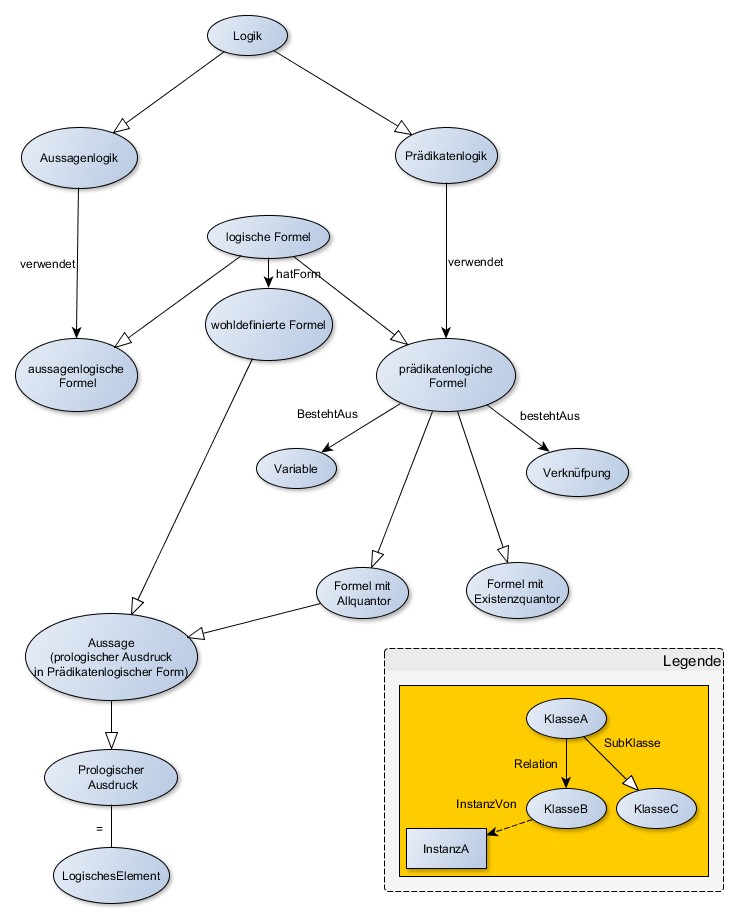
\includegraphics{bilder/formel_baum.png}}}
\caption{Vereinfachte Darstellung von Logik, rein mittels Klassen.\label{fig:prolog_logik_baum}\protect\footnotemark}
\end{figure}
\footnotetext{Eigene Darstellung mittels yEd.}

Um auch Relationen abbilden zu können wurde die Modellierung schliesslich mit Individuen erweitert. Dies erlaubte die Definition von Relationen zwischen diesen, was sich als Schritt in die richtige Richtung erweisen sollte.

\begin{figure}[H]
\centering \rotatebox{0}{\scalebox{0.3}[0.3]{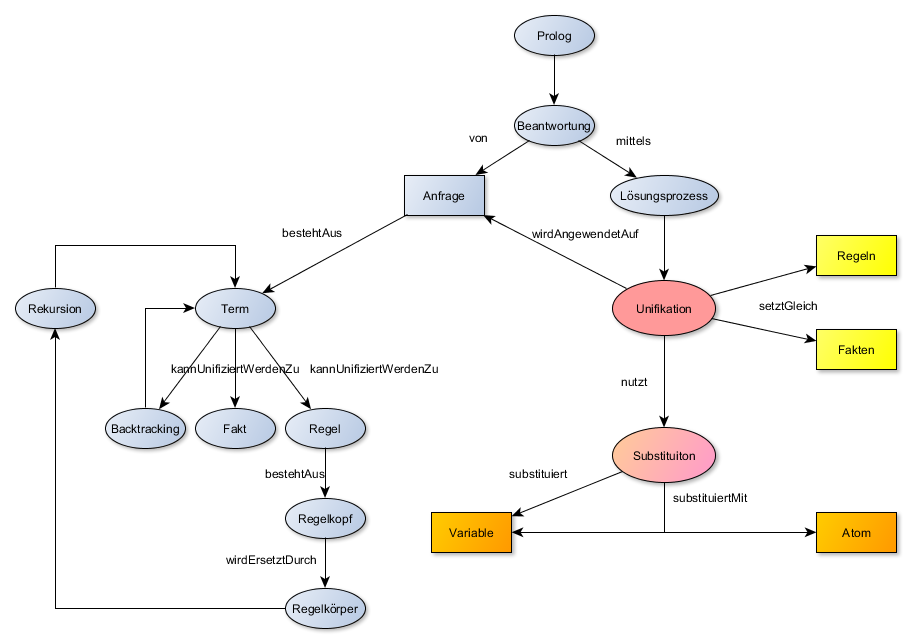
\includegraphics{bilder/loesungsprozess_baum.png}}}
\caption{Vereinfachte Darstellung eines Teils des Lösungsprozesses von Prolog, mittels Klassen, Individuen und Relation.\label{fig:prolog_loesungsprozess}\protect\footnotemark}
\end{figure}
\footnotetext{Eigene Darstellung mittels yEd.}

Es wurde dann jeweils versucht konkrete Fragen aufgrund der erstellten Ontologie zu beantworten, wodurch Mängel in der Ontologie relativ gut sichtbar wurden. Dies konnten dann schrittweise korrigiert werden, so dass die gewünschten Abfragen doch umgesetzt werden konnten. Details zu den gemachten Abfragen finden sich unter~\autoref{sec:anhang:sparql_beispiele}.

\begin{figure}[H]
\centering \rotatebox{0}{\scalebox{0.6}[0.6]{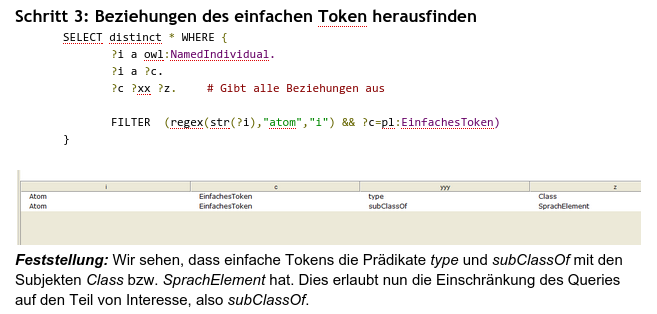
\includegraphics{bilder/sparql_beispiel.png}}}
\caption{Beispiel einer Abfrage der Ontologie mittels SPARQL.\label{fig:sparql_beispiel}\protect\footnotemark}
\end{figure}
\footnotetext{Eigene Darstellung mittels Stanford Protégé und Google Docs.}

Schnell wurde klar, dass solch eine Modellierung ins Uferlose gehen kann, woraufhin der Betreuer der Arbeit, Herr Dr.\ Eckerle, empfahl Literatur über Prolog als Grundlage bzw.\ Rahmen zu verwenden. Hierbei wurde auf das Buch \textit{Künstliche Intelligenz} von \textit{U. Lämmel} und \textit{J. Cleeve} zurückgegriffen~\cite{laemmel}. Daraus resultierte eine verbesserte Modellierung der Ontologie von Prolog, mit Klassen, Relationen und Individuen.

\begin{figure}[H]
\centering \rotatebox{0}{\scalebox{0.15}[0.15]{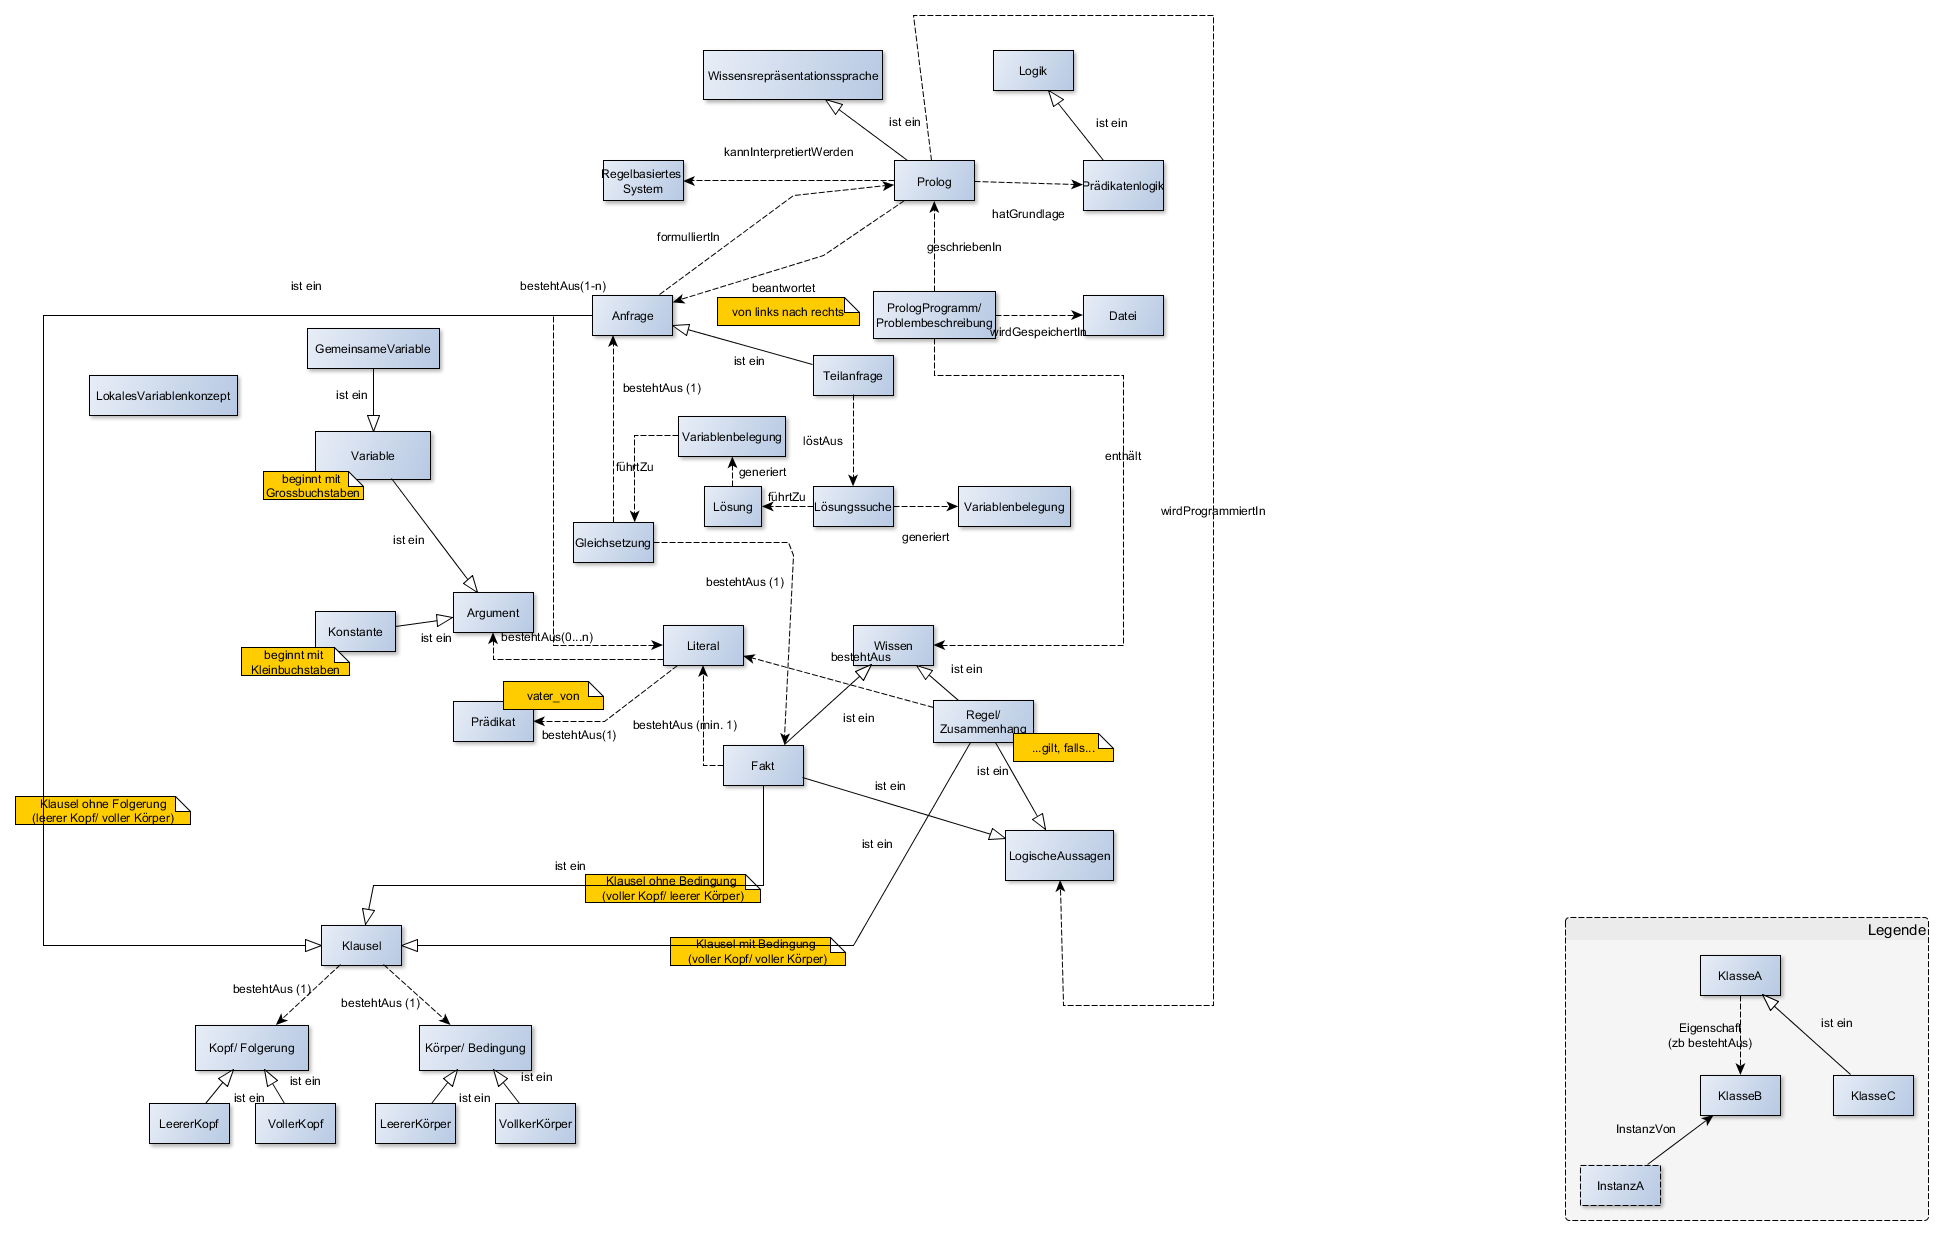
\includegraphics{bilder/prolog_baum.png}}}
\caption{Vereinfachte Darstellung von Prolog, mit Klassen und Relationen (Individuen wurden der Übersicht halber bewusst weggelassen).\label{fig:prolog_baum}\protect\footnotemark}
\end{figure}
\footnotetext{Eigene Darstellung mittels yEd.}

Dies erlaubte jedoch nach wie vor keinen zusätzlichen Gewinn von Mehrwert in Form von Inferenz. Nach diversen Gesprächen mit dem Betreuer der Arbeit, Herrn Dr.\ Eckerle, stellte sich heraus, dass der Ontologie Regeln fehlen. Es wurde dann versucht mithilfe von Prolog das Konzept von Prolog abzubilden. Die Idee dahinter war, von der objektorientierten Denkweise loszukommen. Für die Autoren war es einfach nachzuvollziehen, dass und wie in Prolog Regeln verwendet werden. In Prolog wird auch schnell deutlich, dass eine Abfrage auf Fakten (ohne Regeln) keinen Mehrwert bringt.


Nach diversen, erfolglosen Versuchen Regeln zu finden, wurde dies zuerst anhand einfacher Modelle, des klassisches des Familienstammbaums, versucht, was schlussendlich auch gelang. Mit diesem simplen Beispiel wurde der Mehrwert einer Wissensmodellierung sogleich erkannt.

\begin{figure}[H]
\centering \rotatebox{0}{\scalebox{0.15}[0.15]{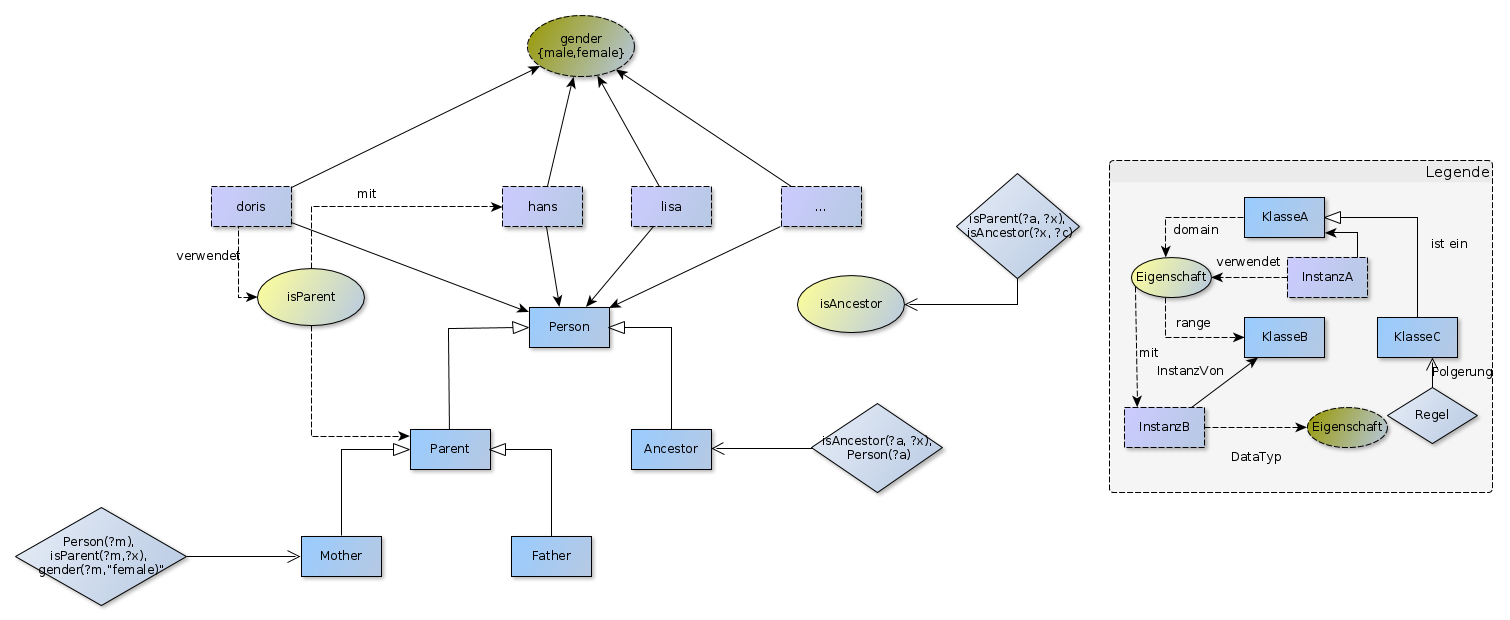
\includegraphics{bilder/familien_netz.png}}}
\caption{Darstellung eines einfachen Beispiels, der Abbildung einer Familie, mit Klassen, Individuen, Relationen und Regeln.\label{fig:familien_netz}\protect\footnotemark}
\end{figure}
\footnotetext{Eigene Darstellung mittels yEd.}

Jedoch gelang es auch nach dieser Erfahrung nicht, Regeln für die eigentliche Wissensdomäne zu finden. Die Erkenntnis aus diesem Prozess ist schlussendlich, dass die Abbildung von Prolog in einer Ontologie zwar möglich ist, jedoch eher in lexikalischer Form, was den Vorteil der Inferenz zunichtemacht. So kann beispielsweise gesagt werden, dass Prolog Unfikikation auf Anfragen anwendet und dabei Regeln mit Fakten gleichsetzt. Dabei wird Substitution genutzt, welche Variablen mit Variablen und/oder Atomen substituiert. Dies wurde aber Grösstenteils in Form von Fakten abgebildet. Einige wenige Regeln konnten erzeugt werden. Das damit abgebildete Wissen könnte aber auf eine einfachere und intuitivere Art mit Fakten abgebildet werden. Somit ist der Mehrwert der Regel nichtig.

\begin{figure}[H]
\centering \rotatebox{0}{\scalebox{0.2}[0.2]{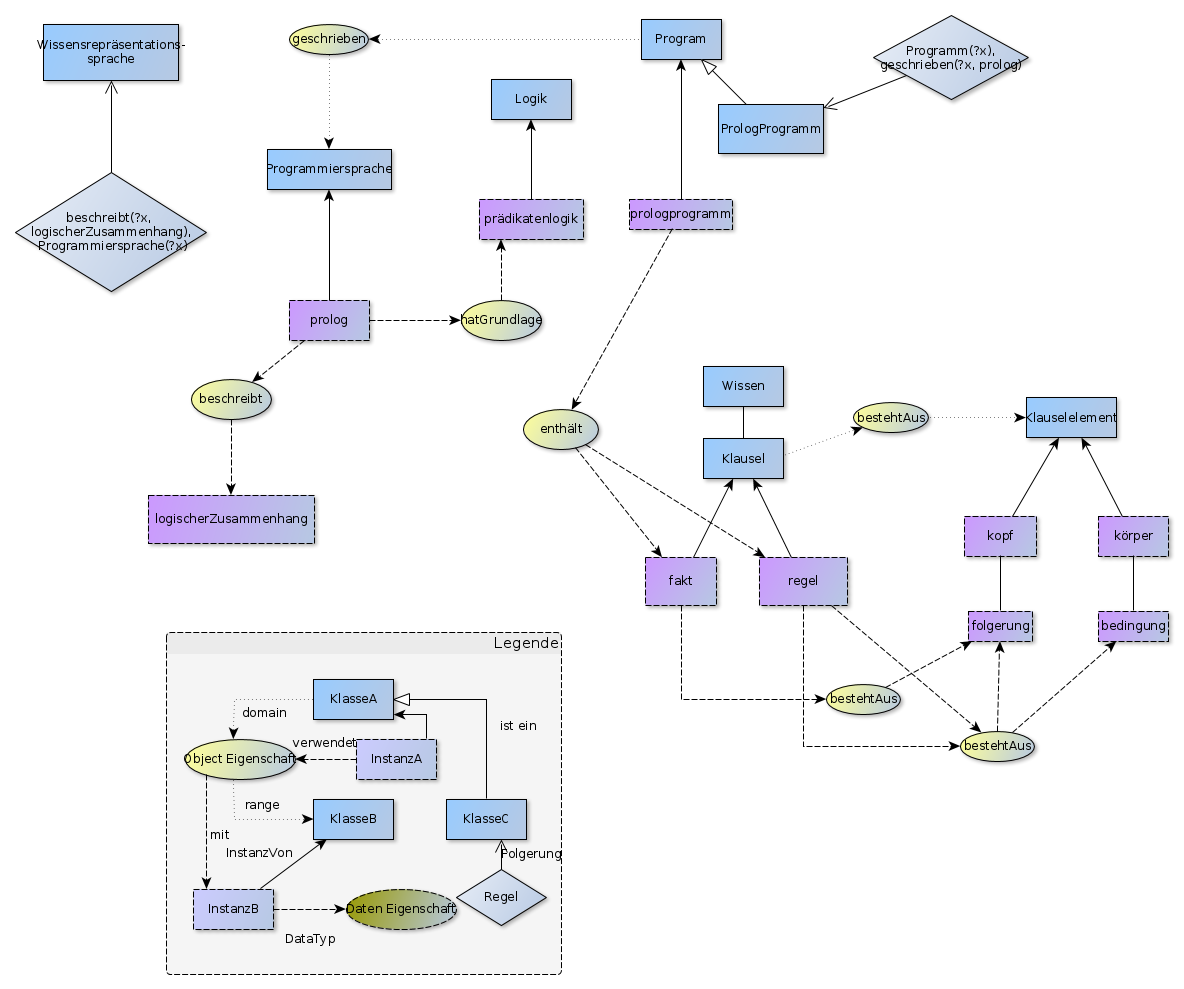
\includegraphics{bilder/prolog_netz.png}}}
\caption{Darstellung eines semantischen Netzes zur Abbildung von Prolog, mit Klassen, Individuen, Relationen und Regeln.\label{fig:prolog_netz}\protect\footnotemark}
\end{figure}
\footnotetext{Eigene Darstellung mittels yEd.}

Nach eingehender Analyse kamen die Autoren zum Schluss das sich die gewählte Domäne nicht eignet um die Mächtigkeit einer Ontologie und dem damit Verbundenen Reasoning abzubilden. Die Wissensmodellierung, besser bekannt als Expertensystemen scheinen sich für Wissensdomänen zu eignen, welche Probleme mit konkreten Objekten Abbilden. Im Gegensatz dazu war die gewählte Domäne Programmiersprache Prolog auf einer zu hohen Abstraktionsebene, als dass der Nutzen sichtbar wird. 

Wie der Name Expertensystem schon andeutet können diese in Fällen verwendet werden,  bei denen zur heutigen Zeit ein Fachexperte notwendig ist, welcher Schlüsse zieht und so die Planung vervollständigt.

Daher wurde eine andere Wissensdomäne --- die Planung von Reisen --- gewählt. Dies geht bereits eher in die Richtung von Expertensystemen, wofür semantische Netze am ehesten geeignet scheinen.

\subsubsection{Modellierung der tatsächlichen Ontologie}
\label{sub:modellierung_der_ontologie_tatsaechliche}

Nach dieser Entscheidung wurde mit der Modellierung also noch einmal beim Punkt null angefangen. Es konnte aber glücklicherweise auf den Erkenntnissen der vorigen Versuchen aufgebaut werden.  

Die Autoren haben mit dem gewonnen Wissen als grundlage entschieden, mithilfe von konkreten Bespielen vorzugehen. Anhand dieser wurde die Ontologie erzeugt und stetig erweitert. Zur Veranschaulichung dazu ein konkretes Beispiel:

\texttt{ Familie Muster plant einen eintägige Ausflug. Die Kinder sind in einem Alter in dem Sie immer beschäftigt sein müssen.}\\

Dies ergab eine noch sehr simple Ontologie, welche mit diesem semantischen Netz abgebildet werden kann:

\begin{figure}[H]
\centering \rotatebox{0}{\scalebox{0.5}[0.5]{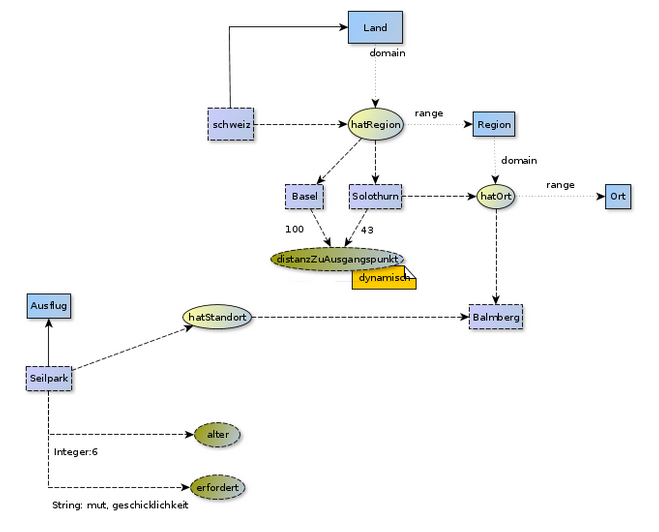
\includegraphics{bilder/famMuster.png}}}
\caption{semantisches Netz für den Tagesausflug von Familie Muster.\label{fig:famMuster}\protect\footnotemark}
\end{figure}
\footnotetext{Eigene Darstellung mittels yEd.}

Mit der neue gewählten Wissensdomäne wurde auch der Sinn hinter der Verwendung von Regeln deutlich:
\begin{figure}[H]
\centering \rotatebox{0}{\scalebox{0.5}[0.5]{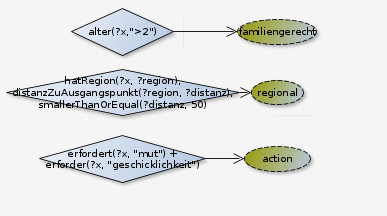
\includegraphics{bilder/famMusterRegeln.png}}}
\caption{Regeln zum semantischen Netz für den Tagesausflug von Familie Muster.\label{fig:famMusterRegeln}\protect\footnotemark}
\end{figure}
\footnotetext{Eigene Darstellung mittels yEd.}

Aus der Modellierung konnten die folgenden Kriterien für die Abfrage abgeleitet werden:

\begin{itemize}
		\item familiengerecht
		\item action
		\item regional
\end{itemize}

Mit der richtigen Sparql abfrage wird der Familie Muster der Seilpark in Balmberg vorgeschlagen.

\begin{lstlisting}
Select * where
	{
		?object :familiengerecht true;
						:regional true;
						:action true.
		}
\end{lstlisting}	


\begin{figure}[H]
\centering \rotatebox{0}{\scalebox{0.5}[0.5]{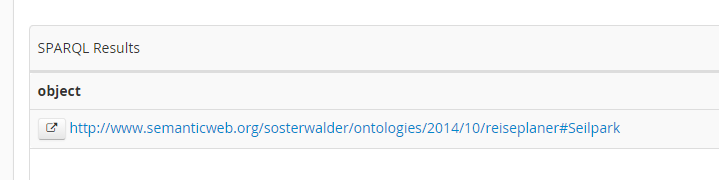
\includegraphics{bilder/famMusterOutput.png}}}
\caption{Ergebnis der Suche von Familie Muster.\label{fig:famMusterOutput}\protect\footnotemark}
\end{figure}
\footnotetext{Eigene Darstellung mittels yEd.}

In diesem ersten sehr einfach gehaltenen Anwendungsfall wird die Herangehensweise der Autoren sichtbar. Im Laufe von weiteren Beispiel wurde die Ontologie erweitert und umgebaut. So haben die Autoren zum Beispiel erst zu einem späteren Zeitpunkt eine Zeiteinheit eingeführt oder gemerkt, dass die Eigenschaft familiengerecht zu oberflächlich und pauschal betrachtet wurde. Diese wurde also noch so umgebaut, dass die Property Subpropertys beinhaltet, welche unterscheidet in welchem alter die Kinder sind. Die gesamte Ontologie wird im Kapitel TODO genauer erläutert.


\subsection{Erstellung der Dokumentation zur Wissensmodellierung }
\label{subsec:dokumentation_wissensmodellierung}
Parallel zur Modellierung der Ontologie entstand eine Dokumentation des Vorgehens zur Wissensmodellierung mit Tutorialcharakter. Diese zeigt exemplarisch auf, wie ein Knowledge Engineer vorgeht, um eine Problemdomäne systematisch zu modellieren und formalisieren. Wie bereits zuvor erwähnt, wurde als Problemdomäne die Planung von Reisen gewählt. Die Dokumentation findet sich unter~\autoref{sec:anhang:tutorial_dokument}.

\subsubsection{Aufbau des Tutorials}
\label{subsec:dokumentation_wissensmodellierung_aufbau}
Im Gegensatz zu herkömmlichen Tutorials enthält das in dieser Arbeit erstellte einen grossen Theorieanteil. Aus diesem Grund wurde das Dokument in drei Teile aufgeteilt. 

Da es sich hierbei um eine wissenschaftliche Arbeit handelt, haben die Autoren entschieden in einem erste Teil  theoretischen Hintergrundwissen zur Wissensmodellierung bereitzustellen. So wird zum Beispiel erläutert was Expertensysteme sind, wie diese graphisch dargestellt werden können und welche Schreibweisen respektive Sprachen verwendet werden um eine Ontologie abzubilden und darauf Abfragen zu stellen.


\noindent\rule[1ex]{\textwidth}{1pt}
\begin{wrapfigure}[2]{l}{0.1\textwidth}
    \vspace{-12pt}
    
\includegraphics[width=0.1\textwidth]{bilder/owl.png}
\end{wrapfigure}
Durch diese Eule wird die zweite Herangehensweise im Dokument eingeleitet. In diesem Teil steht der Fokus auf praktischen Tipps der Autoren. Auf Erfahrungen welche gemacht wurden und mit Mehrwissen hätten vermieden werden können. Die Autoren versuchen dem Leser so die Arbeit zu vereinfachen.

\noindent\rule[1ex]{\textwidth}{1pt}
\begin{wrapfigure}[4]{l}{0.1\textwidth}
    \vspace{-12pt}
    
\includegraphics[width=0.1\textwidth]{bilder/elephant.png}
\end{wrapfigure}
Der letzte Teil des Dokuments, welcher durch den Elefanten gekennzeichnet ist, verkörpert das klassische Tutorial. Einem pragmatisch veranlagten Lesen ist es möglich durch folgen der Eule innerhalb von kurzer Zeit ein simples Beispielexpertensystem aufzubauen.

\subsection{Erarbeitung der praktischen Grundlagen}
\label{subsec:praktische_grundlagen}

Die Erarbeitung der praktischen Grundlage war die Vorarbeit für die Erstellung des Tutorialdokuemnts. Dem entsprechend wurden die gewonnen Erkenntnisse darin eingeflochten.

\subsection{Erstellung der abschliessenden Dokumentation}
\label{subsec:abschliessende_dokumentation}
Mit der Erstellung der abschliessenden Dokumentation ist das hier vorliegende Dokument gemeint.
